%%%%
%       _  _____  ___  _____  _   _  ___ 
%      / \|_   _||_ _||_   _|| | | |/ __|
%     / △ \ | |   | |   | |  | |_| |\__ \
%    /_/¯\_\|_|  |___|  |_|   \___/ |___/
%                 EDUCAÇÃO
%    Modelo de TCC - Ciência da Computação
%%%%

\documentclass[12pt]{article}

\usepackage{sbc-template}
\usepackage{graphicx, url}
\usepackage[utf8x]{inputenc}
\usepackage[brazil]{babel}
\usepackage[T1]{fontenc}
\usepackage[english=american]{csquotes}
\usepackage{float}
\usepackage{comment}
\usepackage{amsmath}
\usepackage{amssymb}
\usepackage{enumerate}
\usepackage{subcaption}
\usepackage{setspace}
\usepackage{listings}
\usepackage{inconsolata}
\usepackage{tabularray}
%\usepackage[backref=page]{hyperref}
%\hypersetup{
%    colorlinks=true,
%    allcolors=blue,
%}

% %%%%%%%%%%%%%%%%%%%%%%%%%%%%%%%%%%%%%%%%%%%%%%%%%%%%%%%%%%%%%%
% define o modelo de referencias
\usepackage[style=abnt]{biblatex}

% indica o arquivo com as referencis bibliograficas
\addbibresource{sbc-template.bib}

% carrega o pacote com alterações para Computação Atitus
\usepackage{sty/cc_atitus}
% %%%%%%%%%%%%%%%%%%%%%%%%%%%%%%%%%%%%%%%%%%%%%%%%%%%%%%%%%%%%%%

% %%%%%%%%%%%%%%%%%%%%%%%%%%%%%%%%%%%%%%%%%%%%%%%%%%%%%%%%%%%%%%
% REFERENCIAS DEVERÃO SER INCLUÍDAS NO ARQUIVO: sbc-template.bib
%
% SOBRE CITAÇÕES:
% Para citar no padrão '(Autores, ano)' use: \cite{chave}
% Para citar no padrão 'Autores (ano)'  use: \textcite{chave} ou \citeonline{chave}
% Para citar no padrão 'Autores'        use: \citelastname{chave}
% Para citar no padrão '(Autor, 2009c; Outro Autor, 2009; Outro Autor, 2015)' use: \cites{chave1}{chave2}{chave3}
% Para citar no padrão 'Autor (ano), Autor (ano) e Autor (ano)' use: \textcites{chave1}{chave2}{chave3}

% Demais exemplos ver documento:
%  https://github.com/abntex/biblatex-abnt/raw/master/doc/biblatex-abnt.pdf
%
% Normas ABNT: https://usp.br/sddarquivos/arquivos/citacoes10520.pdf
%              https://usp.br/sddarquivos/arquivos/abnt6023.pdf
%
% %%%%%%%%%%%%%%%%%%%%%%%%%%%%%%%%%%%%%%%%%%%%%%%%%%%%%%%%%%%%%%
% Atualizações no modelo
% 2024-09-23: (fahadkalil) Ajuste para quebra automática de linhas nas células de uma tabela
% 2024-10-17: (fahadkalil) Inserção de comentários com outras citações e indicação de uso do comando "\enquote"
% %%%%%%%%%%%%%%%%%%%%%%%%%%%%%%%%%%%%%%%%%%%%%%%%%%%%%%%%%%%%%%
% CABEÇALHO
\title{Uso de Redes Neurais em Grafos para Otimização de Tempo no Algoritmo IMOPSO de Maximização de Influência} % titulo

\author{Ana Luiza Almeida Soares\inst{1}, Rodrigo César Pedrosa Silva\inst{1}} % autor principal, orientador

\address{Programa de Pós-Graduação em Ciência da Computação \\ Departamento de Computação \\ Universidade Federal de Ouro Preto
\email{ana.almeida3@aluno.ufop.edu.br, rodrigo.silva@ufop.edu.br}
}
% %%%%%%%%%%%%%%%%%%%%%%%%%%%%%%%%%%%%%%%%%%%%%%%%%%%%%%%%%%%%%%

\begin{document}
\maketitle % Não remova essa linha!

% \begin{abstract} % resumo em inglês
%   Escreva seu resumo em língua estrangeira (inglês)...
% \end{abstract}
     
% \begin{resumo}
%   Resumo do trabalho (português)...  
% \end{resumo}

\section{Introdução}

O problema de Maximização de Influência busca identificar o conjunto de pessoas que maximiza a propagação de influência em uma rede social. Em outras palavras, considerando uma rede social onde os nós representam pessoas e as arestas indicam o nível de influência que uma pessoa exerce sobre outra, o objetivo é encontrar o conjunto de nós que maximize o número de outros nós influenciados.

Esse problema possui inúmeras aplicações, desde a divulgação de produtos em redes sociais até a análise da eficácia da disseminação de informações políticas. O campo vem sendo amplamente estudado devido ao impacto significativo que as redes sociais digitais exercem na formação da opinião pública.

A solução ideal para o problema envolveria avaliar todas as permutações possíveis de conjuntos, mas isso é inviável para redes grandes, devido ao tempo necessário para construir e comparar cada permutação em busca da melhor. 

Consequentemente, várias abordagens foram desenvolvidas. A maioria dessas soluções considera o tamanho do conjunto de influenciadores como um valor fixo, ou seja, a quantidade de pessoas escolhidas para influenciar é uma entrada do algoritmo. Essa abordagem, no entanto, limita a aplicação dessas soluções, já que nem sempre é possível determinar previamente quantos nós devem ser escolhidos, sendo o custo da escolha desses nós, em geral, o principal limitador. Para contornar essa limitação, algumas soluções permitem que o tamanho do conjunto seja variável, impondo uma restrição de custo que se adequa a um orçamento específico, passado como parâmetro ao modelo.

Uma dessas soluções é o algoritmo IMOPSO, que utiliza otimização por enxame de partículas (swarm optimization) e busca local para encontrar uma solução próxima da ótima. Como esse algoritmo emprega heurísticas, ele não garante a solução exata, mas tem apresentado excelentes resultados, especialmente para redes maiores, com uma considerável economia de tempo.

O projeto propõe uma melhoria nesse modelo ao introduzir uma etapa de pré-seleção de nós relevantes para a avaliação. Esses nós serão identificados por uma rede neural de grafos (Graph Neural Network, GNN) com base nas informações derivadas de alguns caminhos mínimos na rede. Essa abordagem busca reduzir o tempo de execução do algoritmo IMOPSO, mantendo sua precisão na solução do problema de Maximização de Influência.

% \section{Referencial Teórico}
% Voltado ao objetivo geral (teoria por trás do método), deve conter os assuntos bases da pesquisa, fazendo citações indiretas e diretas curtas.

% \begin{comment}
% testando comentario
% \end{comment}

% \begin{description}
%     \item[Exemplos de citação indireta]    
% \end{description}

% Segundo \textcite{spinello2024}, o trabalho de conclusão deve ter citações retiradas de artigos científicos encontrados nas bases de dados. 

% O trabalho de conclusão deve ter citações retiradas de artigos científicos encontrados nas bases de dados \cite{spinello2024}.

% \begin{description}
%     \item[Exemplos de citação direta curta]
% \end{description}

% Segundo \textcite{spinello2024} \enquote{o trabalho de conclusão deve ter citações retiradas de artigos científicos encontrados nas bases de dados}. Note que para colocar um texto entre aspas, usamos o comando \verb|\enquote{texto}|.

% Ressalta-se que o \enquote{trabalho de conclusão deve ter citações retiradas de artigos científicos encontrados nas bases de dados} \cite{spinello2024}.

% No estudo comparativo apresentado em \textcite[p. 107]{rabello2010} ...

% No trabalho de \textcite{pargaonkar2021} ...

% Nos trabalhos de \textcites{badgujar2024}{pargaonkar2021} são aplicadas técnicas de ...

% No artigo de \textcite{estevao2023} ...

% \textsc{Citação direta longa devem ser evitadas em artigos científicos!}

% \section{Trabalhos Relacionados}

% Trabalhos semelhantes aos objetivos específicos, sempre detalhando ao final da seção a
% diferença ao trabalho proposto (quantidade -- 5 trabalhos);

% Neste item serão apresentados os principais trabalhos que possuem uma relação com o assunto definido neste estudo....

% % Itens com marcadores
% \begin{itemize}
%      \item \textbf{Título do artigo 01 \cite{ogliari2019}}
     
%      Primeiro parágrafo indicar uma introdução do assunto... \\
%      No segundo: o que o estudo procurou analisar, qual o objetivo... \\
%      No terceiro: o que foi desenvolvido, qual aplicação/experimento foi realizado... \\
%      Último: em quais conclusões o trabalho chegou... \\
         
%     \item \textbf{Título do artigo 02 (Autor, ano)}
    
%      Primeiro parágrafo indicar uma introdução do assunto... \\
%      No segundo: o que o estudo procurou analisar, qual o objetivo... \\
%      No terceiro: o que foi desenvolvido, qual aplicação/experimento foi realizado... \\
%      Último: em quais conclusões o trabalho chegou... \\
    
%     \item \ldots
% \end{itemize}

\section{Materiais e Métodos}
    Tecnologias, instrumentos e procedimentos que serão usados no estudo. O Algoritmo \ref{alg:id_algo} se refere ao método de ordenação Bubblesort expresso em linguagem Python.

    % Código-fonte formatado
    % Ver: https://en.wikibooks.org/wiki/LaTeX/Source_Code_Listings
    \begin{lstlisting}[  
        %float,
        language=Python, 
        frame=single, 
        numbers=left,
        caption={Método de ordenação Bubblesort},
        label={alg:id_algo} % id para referenciar
        ]        
    def bubble_sort(alist):
        for i in range(len(alist)-1,0,-1):
            for j in range(i):
                if alist[i]>alist[i+1]:
                    temp = alist[i]
                    alist[i] = alist[i+1]
                    alist[i+1] = temp    
    \end{lstlisting}

    % Figura
    % https://pt.overleaf.com/learn/latex/Inserting_Images
    \begin{figure}[H]
        \centering
        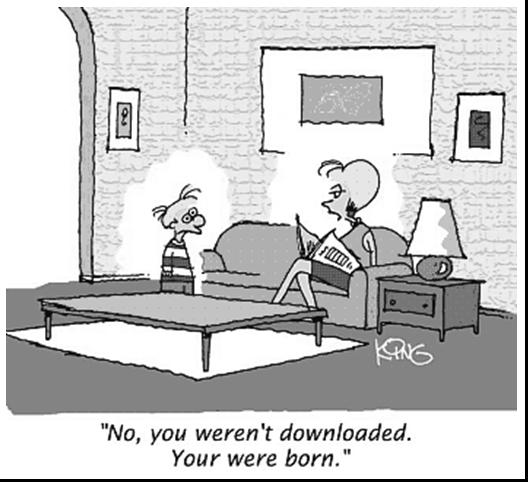
\includegraphics[width=0.5\textwidth]{fig1.jpg}
        \caption{Minha figura}
        \label{fig:id_figura}
    \end{figure}
    
    % Tabela
    % Editor online: https://www.latex-tables.com
     \begin{table}[ht]
        \centering
        \caption{Minha tabela}
        \label{tab:id_tabela}
        \begin{tblr}{
          colspec = {X[l] X[l]}, % Tipo X define células com quebra automática de linha. Use: l=left, r=right, c=center ou j=justify para alinhamento dentro das células
          width = \linewidth,
          hlines, % inclui borda horizontal
          vlines, % inclui borda vertical        
        }
        \textbf{cabeçalho 1} & \textbf{cabeçalho 2} \\
        {texto à esquerda} & {Existem muitas variações das passagens do Lorem Ipsum disponíveis, mas a maior parte sofreu alterações de alguma forma, pela injecção de humor, ou de palavras aleatórias que nem sequer parecem suficientemente credíveis. Se vai usar uma passagem do Lorem Ipsum, deve ter a certeza que não contém nada de embaraçoso escondido no meio do texto.}
        \end{tblr}
    \end{table}

\section{Resultados Esperados}
Essa seção deverá ser escrita na segunda parte do trabalho, conhecida como TCC2.

% \section{Considerações Finais}
% Essa seção deverá ser escrita na segunda parte do trabalho, conhecida como TCC2.

% %%%%%%%%%%%%%%%%%%%%%%%%%%%%%%%%%%%%%%%%%%%%%%%%%%%%%%%%%%%%%%
% Seção de Referências (gerada automaticamente)
\printbibliography  % Não remover esta linha
% %%%%%%%%%%%%%%%%%%%%%%%%%%%%%%%%%%%%%%%%%%%%%%%%%%%%%%%%%%%%%%

\end{document}